The \textit{Drawing Study} is designed to be of exploratory nature. This means that the research question it aims to answer is not as concrete as for instance the one of our \textit{Evaluation Study}. The goal is to gain insights into the intuitiveness of visual encodings and to find out how people would visualize temporal uncertainty by themselves. This information could consequently be used in the design of novel visualizations, aimed at expert and especially non-expert users. \par \medskip

To gain these insights, we describe predefined scenarios, which encompass some kind of temporal uncertainty, to our study participants and ask them to draw a visualization sketch that intuitively represents this given scenario. Furthermore, the participants are always provided with a certain task a hypothetical user should be able to efficiently solve given an implementation of the sketched design. \par \medskip

To elicit the desired sketches of temporal visualizations from our study participants, we have to ask the right questions and also have to pay close attention to ask them in the right way. This means that it is imperative to not suggest any possible answers or solution approaches while communicating the task that should be solved, because this would greatly affect their given answers \cite{hullman2016evaluating}. For this reason we try our best to make the given scenario and the task as clear as possible to our participant without suggesting anything that would help in the solution of the task. \par \medskip

The scenarios and task are chosen to be as representative as possible to many typical tasks that can be solved through the visualization of uncertainties. This specification matches the one we already had for our \textit{Evaluation Study}. Hence, we use the same 4 main types of tasks:
\begin{enumerate}
	\item The first task is to create a visualization that makes it possible to gauge the probability of something for a given point in time in the uncertainty interval. The concrete scenario text to be visualized is as follows: ''\textit{A bus should arrive at 12:00, but may be running late for up to 10 minutes. How would you visualize this scenario, so that you can estimate the probability of still catching the bus if you arrive at the bus station at a given point in time?}''. Figure \ref{fig:drawingT1} shows an example sketch for this scenario.
	
	\begin{figure}[H]
		\begin{minipage}{.45\textwidth}
			\centering
			\captionsetup{width=0.8\textwidth}
			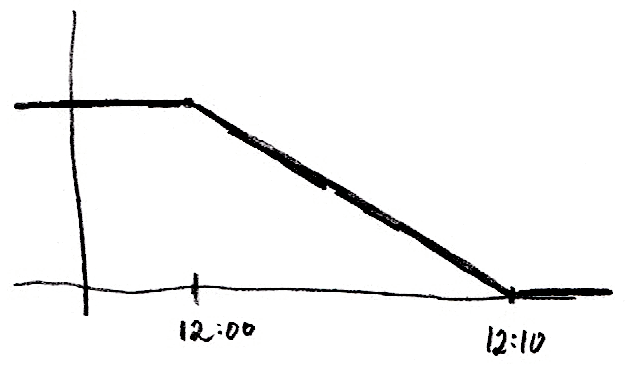
\includegraphics[height=0.5\textwidth]{figures/drawingT1.png}
			\caption{\textit{TODO}}
			\label{fig:drawingT1}
		\end{minipage}
		\begin{minipage}{.45\textwidth}
			\centering
			\captionsetup{width=0.8\textwidth}
			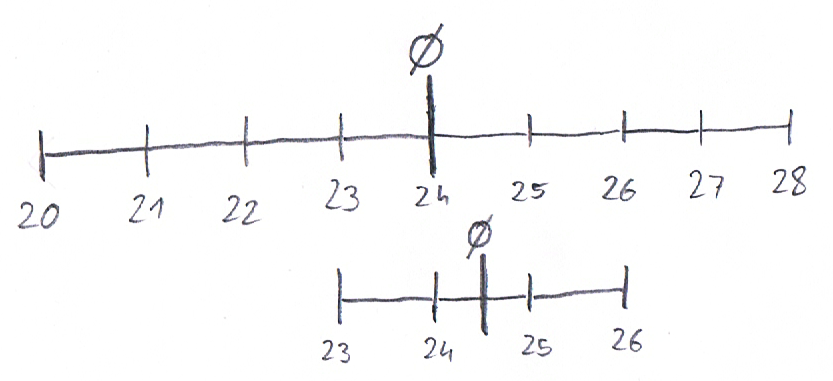
\includegraphics[height=0.5\textwidth]{figures/drawingT2.png}
			\caption{\textit{TODO}}
			\label{fig:drawingT2}
		\end{minipage}
	\end{figure}
	
	\item The second task is about the comparison of two given uncertain end times of intervals. The task is to judge which of the two intervals will end earlier on average. The concrete scenario text is as follows: ''\textit{There are two possible approaches to a given project. The first approach will take 20 to 28 days, while the second one will take 23 to 26 days. How would you visualize the scenario, so you can effectively judge which of the two approaches will on average lead to an earlier completion of the project?}''. Figure \ref{fig:drawingT2} shows an example sketch for this scenario.
	
	\item The third task works with the same scenario as the second one and only adapts the user task that the visualization should support. Instead of judging the overall average completion time, the user should be able to make a decision which approach is better to finish the project until a given date. In other words, the user has to compare the completion probability of both approaches in a given point in time. This scenario usually did not lead to helpful answers or additional sketches, but more on that in the \hyperref[ch:discussion]{Discussion Chapter}.
	
	\item The fourth and last task of the study is about judging the probability of an overlap of two uncertain events. One of the given events has an uncertain end time, while the other event start within an uncertain time frame. The concrete scenario is as follows: ''\textit{Two lectures are taking place after each other. the first lecture will end between 11:50 and 12:05, while the second lecture will start between 12:00 and 12:15. How would you visualize this scenario to be able to judge the probability of an overlap of the two lectures? Furthermore, it should be possible to accurately judge the interval in which an overlap can possible take place from your visualization.}''. Figure \ref{fig:drawingT4} shows an example sketch for this scenario.
	
	\begin{figure}[H]
		\centering
		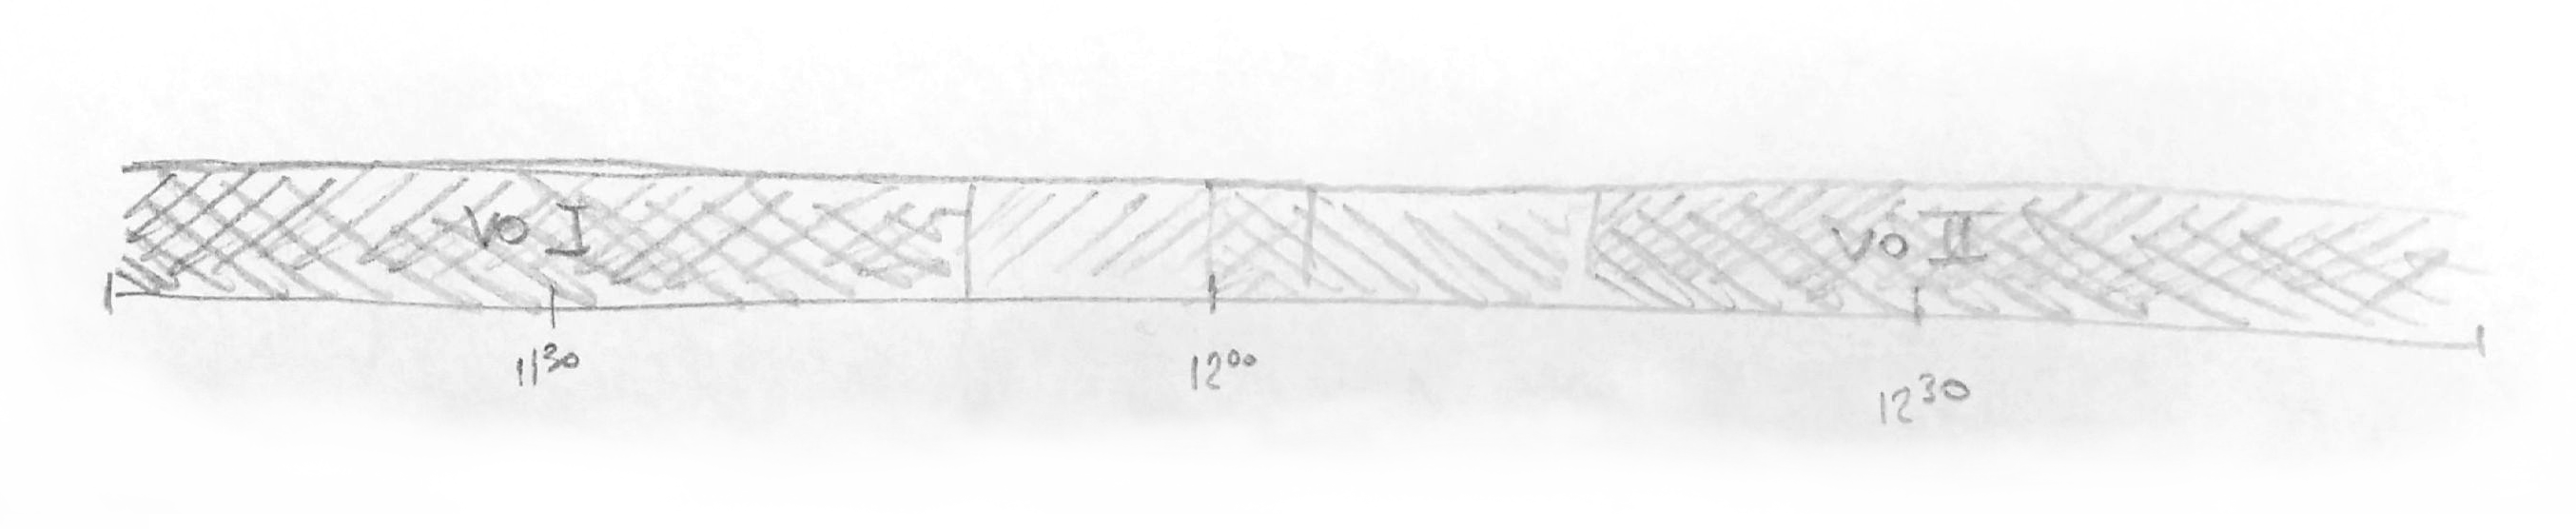
\includegraphics[width=0.75\textwidth]{figures/drawingT4.png}
		\caption{\textit{TODO}}
		\label{fig:drawingT4}
	\end{figure}
\end{enumerate} 

TODO intro zu den szenarios
TODO wir lesen die aufgaben nicht nur vor sonder erklären sie auch